\documentclass[10pt,a4paper]{article}
\usepackage[utf8]{inputenc}
\usepackage{graphicx}
\usepackage{paracol}
\usepackage{geometry}
\usepackage{hyperref}
\usepackage[dvipsnames]{xcolor}
\usepackage{titlesec}
\usepackage{fontawesome}
\usepackage{url}
\usepackage{microtype}
\usepackage{xurl}

\geometry{a4paper, margin=0.5in, top=0.5in, bottom=0.5in}

\hypersetup{
    colorlinks=true,
    linkcolor=blue,
    filecolor=magenta,
    urlcolor=cyan,
}

\definecolor{titlegrey}{gray}{0.4}
\definecolor{textgrey}{gray}{0.3}
\definecolor{sectioncolor}{gray}{0.6}

\titleformat{\section}{\color{sectioncolor}\large\bfseries}{}{0em}{}[\titlerule]
\titlespacing*{\section}{0pt}{1.5ex plus 1ex minus .2ex}{1.5ex plus .2ex}

\renewcommand{\familydefault}{\sfdefault}

\begin{document}

\pagestyle{empty}

\begin{center}
    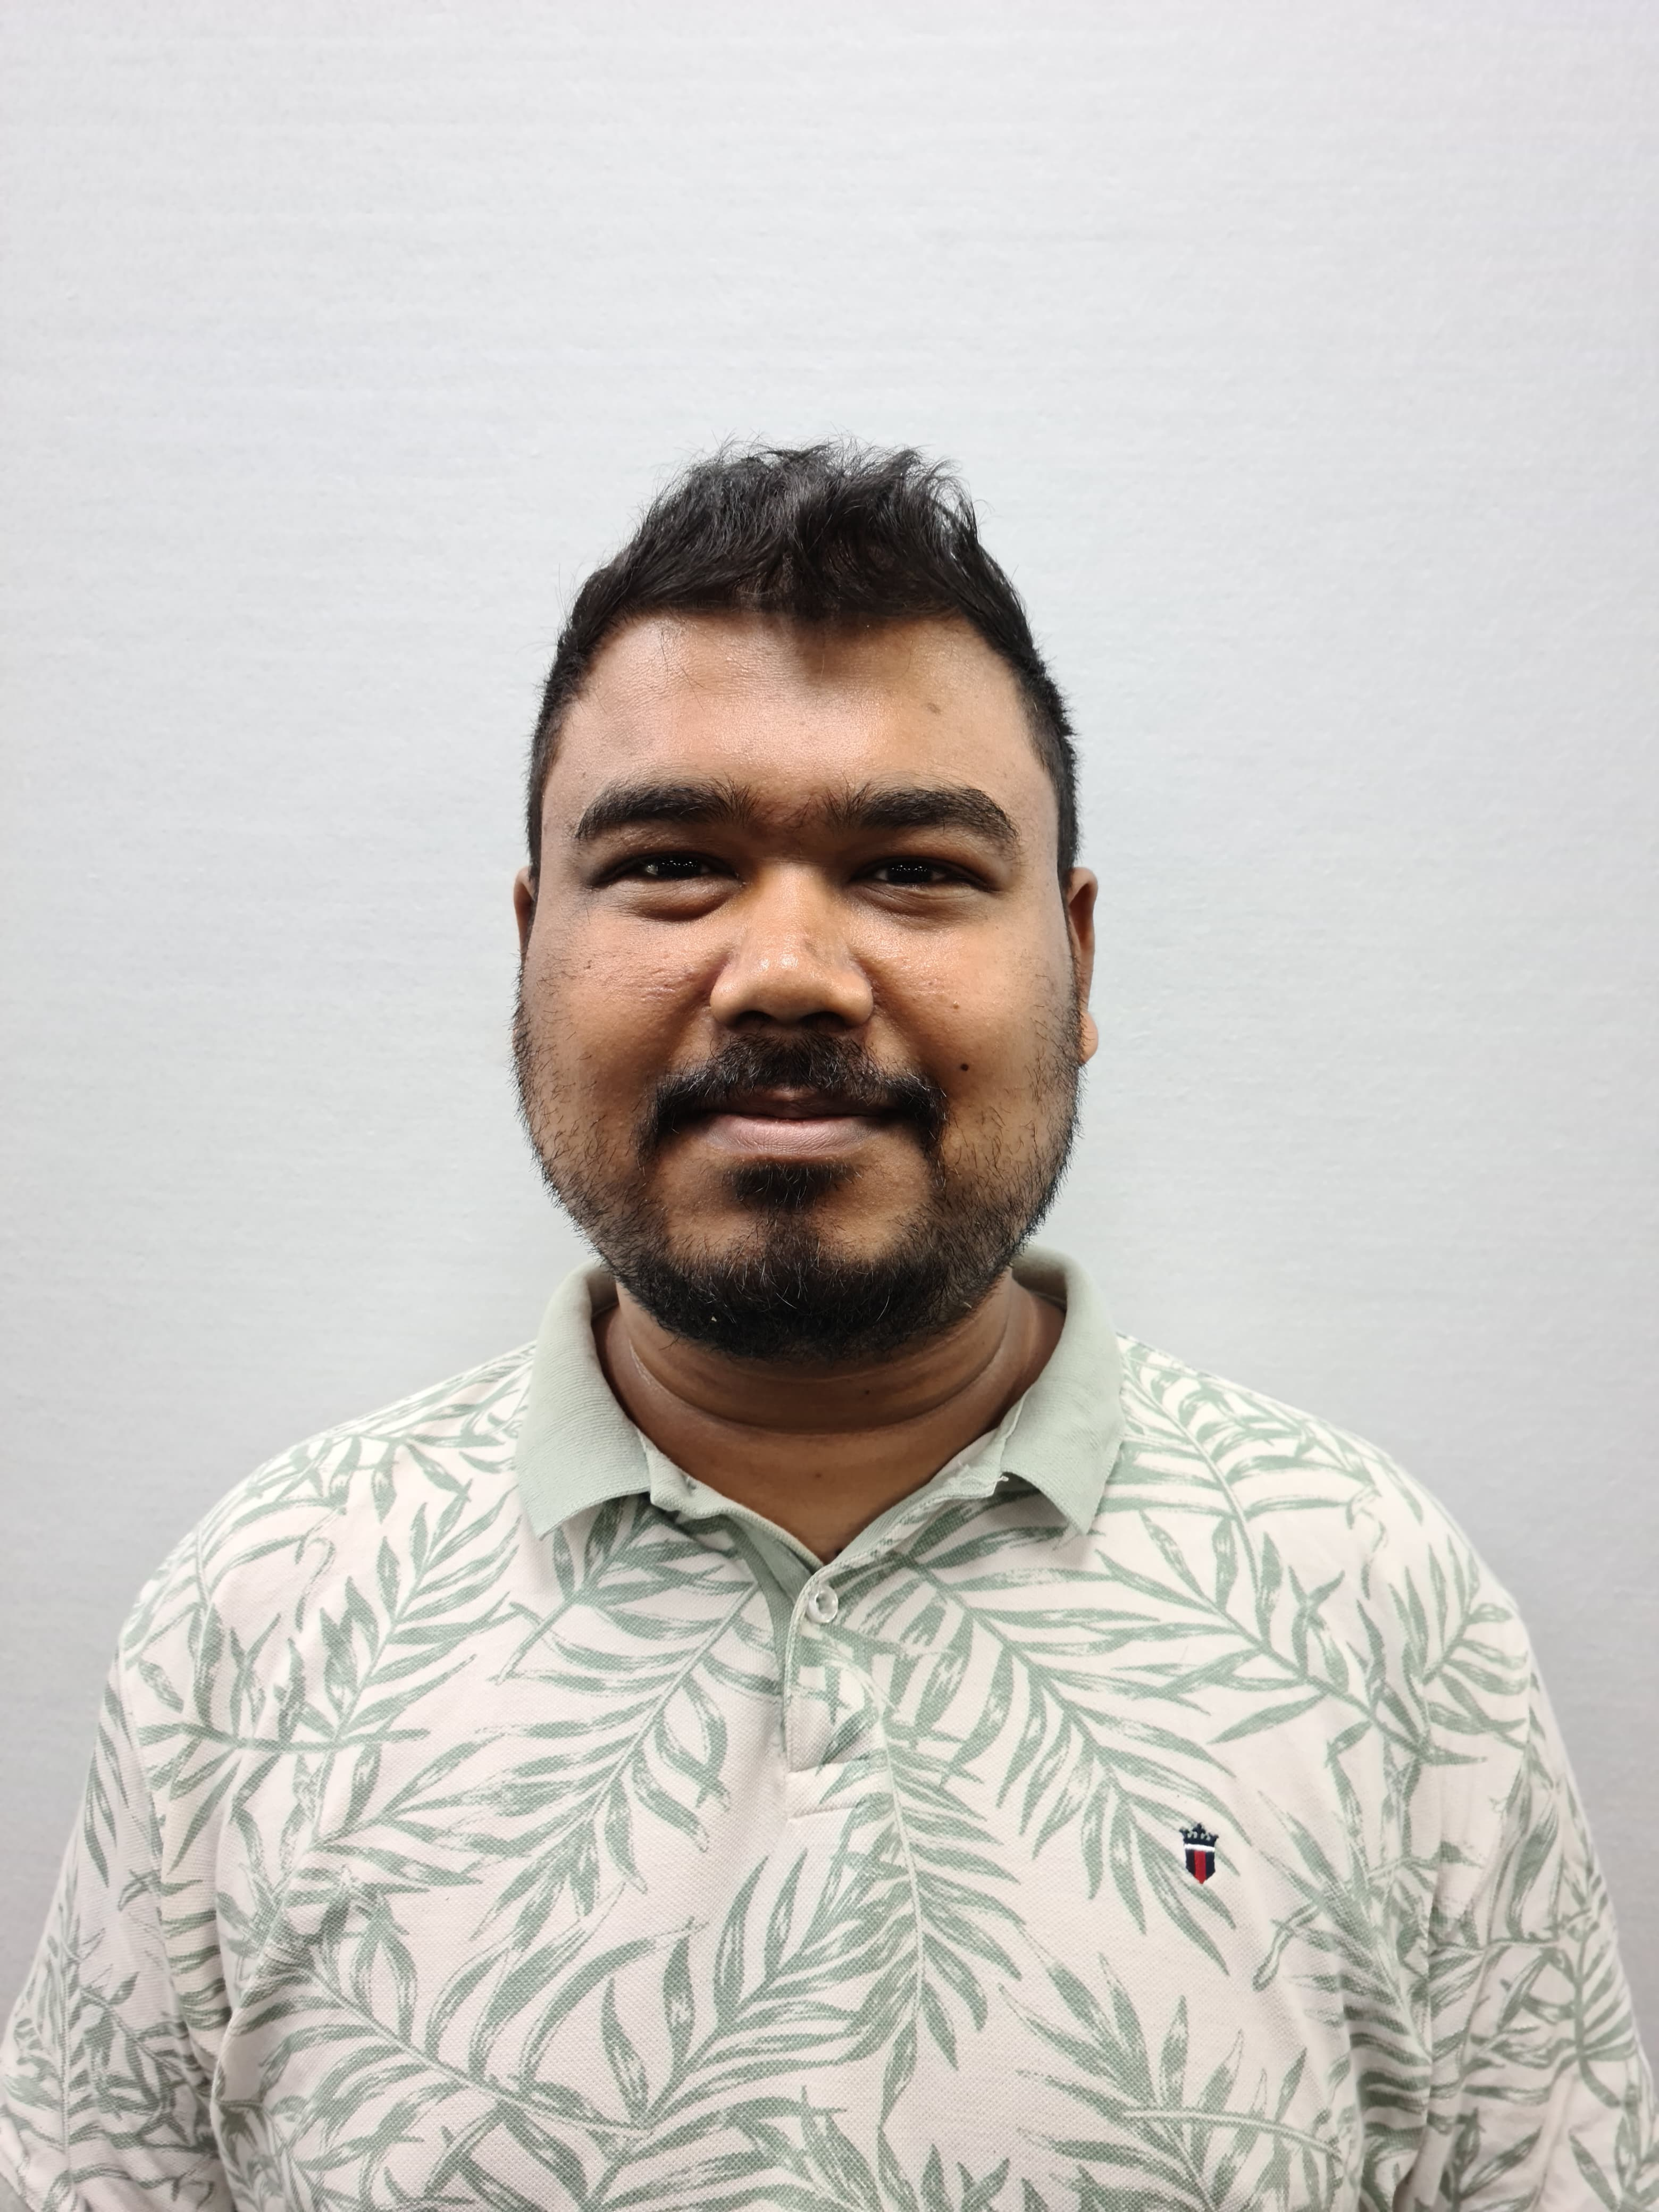
\includegraphics[width=0.12\textwidth,height=0.12\textwidth,keepaspectratio,clip]{passport_photo.jpeg} \\
    \vspace{3mm}
    {\Huge \textbf{Biswadeep Baruah}} \\
    \vspace{2mm}
    {\Large \color{titlegrey} Software Developer}
\end{center}
\vspace{5mm}

\begin{paracol}{2}
\begin{leftcolumn}

\section*{About me}
\textcolor{textgrey}{
Highly skilled backend developer with a strong proficiency in Python and Laravel, offering a Year of experience in creating efficient and scalable solutions. Seeking a challenging role to leverage my expertise and contribute to the success of a dynamic organization.
}

\section*{Personal}
\textcolor{textgrey}{
\begin{tabular}{@{}p{0.9\linewidth}}
    \textbf{Biswadeep Baruah} \\
    Fauzdaripatty b.bora road, P.O: Haibargaon, Dist.: Nagaon, Assam-782002 \\
    \textbf{Phone:} +91 7002615821 \\
    \textbf{Email:} bswbrh3@gmail.com \\
\end{tabular}
}

\section*{Areas of specialization}
\textcolor{textgrey}{
\begin{itemize}
    \item Backend Developer
    \item Python
    \item PHP
\end{itemize}
}

\section*{Interests}
\textcolor{textgrey}{
\begin{itemize}
    \item \textbf{Video Games:} I’m all about strategic gaming.
    \item \textbf{Guitar and music:} When I am having good times with friends.
\end{itemize}
}

\section*{Degrees}
\textcolor{textgrey}{
\begin{itemize}
    \item \textbf{2022 MTECH} - University of Hyderabad - CGPA: 81.30 \hfill 
\includegraphics[width=0.06\textwidth,height=0.06\textwidth,keepaspectratio]{uoh.png}
    \item \textbf{2018 BTECH} - Jorhat Engineering College - CGPA: 66.00 \hfill 
\includegraphics[width=0.06\textwidth,height=0.06\textwidth,keepaspectratio]{JEC_logo.jpg}
    \item \textbf{2013 HSSLC} - Vikas Vidyaniketan - Percentage: 81.00 \hfill 
\includegraphics[width=0.06\textwidth,height=0.06\textwidth,keepaspectratio]{VIKAS.png}
    \item \textbf{2011 HSLC} - Christ Jyoti School - Percentage: 69.00 \hfill 
\includegraphics[width=0.06\textwidth,height=0.06\textwidth,keepaspectratio]{CJS.png}
\end{itemize}
}

\section*{Skills}
\textcolor{textgrey}{
\begin{itemize}
    \item Python, PHP
    \item Flask, Laravel
    \item MySQL, MongoDB
    \item Git, Postman
\end{itemize}
}

\section*{Achievements}
\textcolor{textgrey}{
\begin{itemize}
    \item \textbf{2023} Rising Star Award for the month of May 2023 at Expand My Business.
    \item \textbf{2011} Anundoram Borooah Award, 2011
    \item \textbf{2008} 37th position in the Maths Olympiad, 2008
\end{itemize}
}

\section*{Languages}
\textcolor{textgrey}{
\begin{itemize}
    \item Assamese (mother tongue)
    \item English
    \item Hindi
\end{itemize}
}

\section*{Social}
\textcolor{textgrey}{
\faGithub\ \href{https://github.com/Biswa17}{Biswa17} \\
\faLinkedin\ \href{https://linkedin.com/in/biswa-baruah}{Biswa Baruah}
}

\end{leftcolumn}

\begin{rightcolumn}

\section*{WORK EXPERIENCE}
\subsection*{Oct 2022–Present Expand My Business \hfill 
\includegraphics[width=0.06\textwidth,height=0.06\textwidth,keepaspectratio]{exmyb.png}}
\subsubsection*{Backend Developer (PHP) | Dates: Feb 2023 - Feb 2024}
\textcolor{textgrey}{
\begin{itemize}
    \item \textbf{Snabbcom (Feb 2023 - May 2023):} Played a key role in the back-end development of an e-commerce website creation platform built on Laravel. Designed and implemented RESTful APIs for seamless frontend and backend communication. Ensured data security and implemented efficient algorithms for optimized system performance.
    \item \textbf{Tata Star Delite and Star Quik (May 2023 - Nov 2023):} Worked on projects for Tata, contributing to successful solutions now live. Involved in backend development tasks to ensure robustness and efficiency. Collaborated with cross-functional teams to meet project goals and deadlines. Implemented Star Quik using microservice architecture, leveraging its benefits for scalability and maintainability. Integrated modern search services from Wizzy for improved search functionality and seamlessly incorporated features like email and SMS integration with various third-party services to deliver a unified and enhanced user experience.
    \item \textbf{Socialee E-commerce App (Sept 2023 - Ongoing):} Contributed to the development of an e-commerce app with a reel feature called Socialee, currently available on the Play Store: \url{https://play.google.com/store/search?q=socialee&c=apps&hl=en_IN&gl=US}. Played a key role in backend development, overseeing various components. Collaborated with UX/UI designers and the Frontend team to optimize the overall user experience. Implemented a sophisticated multi-country and multi-language feature supporting both Arabic and English, facilitating delivery across Dubai, Riyadh, and India. Introduced a unique earning model, allowing content creators to monetize their work by earning a commission for each sale generated through their created content.
\end{itemize}
}

\subsubsection*{Backend Developer (Python) | Dates: Oct 2022 - Feb 2023}
\textcolor{textgrey}{
\begin{itemize}
    \item \textbf{Expand My Business Development:} Contributed to the back-end development of Expand My Business, a marketplace connecting vendors and clients for B2B projects across various verticals, including e-commerce, ERP, gaming, digital marketing, and other digital needs. Developed robust and scalable features using Python to enhance the marketplace platform. Collaborated with cross-functional teams, including sales, marketing, and delivery, to gather requirements and implement efficient backend solutions. Utilized an internally developed project management tool, built with Python, for effective team coordination and project tracking. Integrated APIs, managed databases, and optimized website performance to ensure a seamless and efficient user experience.
\end{itemize}
}

\section*{PROJECTS}
\textcolor{textgrey}{
\begin{itemize}
    \item \textbf{2016 Regional Transport Office Vehicle Registration System:}
    \begin{itemize}
        \item Designed and developed a streamlined vehicle registration system for the Btech project.
        \item Implemented data validation, user authentication, and efficient database management.
    \end{itemize}
    \item \textbf{2018 Parallel Programming Optimization:}
    \begin{itemize}
        \item Employed parallel programming techniques to enhance program efficiency.
    \end{itemize}
    \item \textbf{2021 Cryptanalysis of Lightweight Block Cipher:}
    \begin{itemize}
        \item Conducted research on a vulnerability in the Twine-80 cipher.
        \item Theoretically identified an exploit that could potentially reduce the time required to break the cipher from $2^{80}$ to $2^{78}$.
    \end{itemize}
\end{itemize}
}

\end{rightcolumn}
\end{paracol}

\vfill
\begin{center}
\textcolor{textgrey}{
\begin{tabular}{c c c}
\faMapMarker\ Assam, Gurgaon & \faPhone\ +91 8011245653 & \faEnvelope\ bswbrh3@gmail.com
\end{tabular}
}
\end{center}

\end{document}
